\section{Нестандартные задачи}
1. Делится ли число $\underbrace{11\ldots11}_{\mbox{{\scriptsize 1998 единиц}}}$: а) на 3; б) на 2; в) на 6.\\
2. Делится ли число $\underbrace{22\ldots22}_{\mbox{{\scriptsize 239 двоек}}}$: а) на 3; б) на 2; в) на 6.\\
3. НОД(a,b)=a. Чему равен НОК (a,b)?\\
4. НОК(a,b)=a. Чему равен НОД (a,b)?\\
5. В классе 35 учеников, из которых 20 занимаются в математическом кружке, 11 --- в кружке <<Умелые руки>>, а 10 ребят в эти кружки не ходят. Сколько математиков занимаются в кружке <<Умелые руки>>?\\
6. В классе 37 учеников, из которых 19 занимаются в физическом кружке, 13 --- в биологическом кружке, а 10 ребят в эти кружки не ходят. Сколько физиков занимаются в биологическом кружке?\\
7. Произведение двух последовательных чётных чисел на 120 меньше произведения двух следующих за ними чётных чисел. Найдите эти числа.\\
8. Произведение двух последовательных нечётных чисел на 144 меньше произведения двух следующих за ними нечётных чисел. Найти эти числа.\\
9. Существуют ли такие натуральные $a$ и $b,$ что $(a+b)(3a-b)=6?$\\
10. Существуют ли такие натуральные $a$ и $b,$ что $(a+b)(3a-b)=10?$\\
11. Из трёхзначного числа вычли сумму его цифр. Может ли разность оказаться равной 189?\\
12. Из трёхзначного числа вычли сумму его цифр. Может ли разность оказаться равной 180?\\
13. Сколько клеток пересекает диагональ в клетчатом прямоугольнике размером $239\times566?$\\
14. Сколько клеток пересекает диагональ в клетчатом прямоугольнике размером $239\times366?$\\
15. Какое наибольшее количество точек пересечения могут иметь 9 окружностей?\\
16. Дана последовательность целых чисел: 0; 1; -1; 2; -2; 3; -3... Какое число будет на 366 месте? На каком месте в этой последовательности встретится число 366?\\
17. Дана последовательность целых чисел: 0; 1; -1; 2; -2; 3; -3... Какое число будет на 239 месте? На каком месте в этой последовательности встретится число 239?\\
18. Известно, что числитель дроби $\cfrac{5k^2+7k+11}{8k^2+6k+2}$ делится на 13. Докажите, что дробь можно сократить на 13.\\
19. Известно, что числитель дроби $\cfrac{3k^2+7k+1}{8k^2+4k+10}$ делится на 11. Докажите, что дробь можно сократить на 11.\\
20. Средний возраст одиннадцати игроков <<Зенита>> --- 22 года. Во время матча один из игроков был удалён и ушёл с поля. Средний возраст оставшихся на поле игроков стал равен 21 году. Сколько лет удалённому футболисту?\\
21. Средний  возраст одиннадцати игроков <<Зенита>> --- 26 лет. Во время матча один из игроков был удалён и ушёл с поля. Средний возраст оставшихся на поле игроков стал равен 25 годам. Сколько лет удалённому футболисту?\\
22. Куплено несколько одинаковых книг и одинаковых тетрадей. За книги заплачено 1072 рубля. Сколько куплено книг, если цена одной книги более чем на 100 рублей превосходит цену тетради, а книг куплено на 6 больше, чем тетрадей? Стоимость книг и тетрадей составляет целое число рублей.\\
23. Куплено несколько одинаковых книг и одинаковых тетрадей. За книги заплачен 1071 рубль. Сколько куплено книг, если цена одной книги более чем на 100 рублей превосходит цену тетради, а книг куплено на 5 больше, чем тетрадей? Стоимость книг и тетрадей составляет целое число рублей.\\
24. На складе имеются 33 коробки массой 19 кг каждая и 27 коробок массой 49 кг каждая. Все эти коробки разложили в два штабеля. Обозначим за $S_1$ и $S_2$ суммарные массы коробок в первом и втором штабеле соответственно, и пусть $A=|S_1-S_2|.$\\
а) Найдите наименьшее возможное значение числа $A,$ если в каждом штабеле находится 30 коробок.\\
б) Может ли $A$ равняться нулю, если коробки распределены по штабелям не обязательно поровну?\\
25. На складе имеются 25 коробок массой 13 кг каждая и 19 коробок массой 29 кг каждая. Все эти коробки разложили в два штабеля. Обозначим за $S_1$ и $S_2$ суммарные массы коробок в первом и втором штабеле соответственно, и пусть $A=|S_1-S_2|.$\\
а) Найдите наименьшее возможное значение числа $A,$ если в каждом штабеле находится 22 коробки.\\
б) Может ли $A$ равняться нулю, если коробки распределены по штабелям не обязательно поровну?\\
26. По кругу каким-то образом расставили все натуральные числа от 1 до 15 (каждое число встречается один раз). Для каждой пары соседних чисел нашли разность большего и меньшего. а) Могли ли все полученные разности быть не меньше 7? б) Могли ли все полученные разности быть не меньше 8? Не забудьте объяснить свой ответ.\\
27. По кругу каким-то образом расставили все натуральные числа от 1 до 17 (каждое число встречается один раз). Для каждой пары соседних чисел нашли разность большего и меньшего. а) Могли ли все полученные разности быть не меньше 8? б) Могли ли все полученные разности быть не меньше 9? Не забудьте объяснить свой ответ.\\
28. Назовём трёхзначное натуральное число {\it хорошим,} если оно кратно трём и первые две его цифры отличаются на единицу. Найдите количество хороших чисел, запись которых заканчивается на 7 или на 8.\\
29. Назовём трёхзначное натуральное число {\it интересным,} если оно кратно трём и первые две его цифры отличаются на два. Найдите количество интересных чисел, запись которых заканчивается на 6 или на 7.\\
30. Имеются каменные глыбы: 50 штук по 700 кг каждая, 60 штук по 1000 кг каждая, 80 штук по 1500 кг каждая. Глыбы нельзя раскалывать. Считается, что глыбы можно погрузить в грузовик, если их общая масса не превосходит грузоподъёмности этого грузовика. а) Докажите, что все эти глыбы можно одновременно погрузить на 44 грузовика грузоподъёмностью 5 тонн каждый. б) Докажите, что все эти глыбы нельзя одновременно погрузить на 43 грузовика грузоподъёмностью 5 тонн каждый.\\
31. Имеются каменные глыбы: 50 штук по 800 кг каждая, 60 штук по 1000 кг каждая, 60 штук по 1500 кг каждая. Глыбы нельзя раскалывать. Считается, что глыбы можно погрузить в грузовик, если их общая масса не превосходит грузоподъёмности этого грузовика. а) Докажите, что все эти глыбы можно одновременно погрузить на 39 грузовиков грузоподъёмностью 5 тонн каждый. б) Докажите, что все эти глыбы нельзя одновременно погрузить на 38 грузовиков грузоподъёмностью 5 тонн каждый.\\
32. При умножении двух натуральных чисел, одно из которых на 10 меньше другого, ученик ошибочно уменьшил цифру десятков произведения на 4. Для проверки ответа он поделил полученное неправильное произведение на меньший множитель и получил в частном 39, а в остатке 22. Какие числа он умножал?\\
33. При умножении двух натуральных чисел, одно из которых на 10 больше другого, ученик ошибочно уменьшил цифру десятков произведения на 6. Для проверки ответа он поделил полученное неправильное произведение на меньший множитель и получил в частном 49, а в остатке 22. Какие числа он умножал?\\
34. Шарики можно разложить в пакетики, а пакетики упаковать в коробки, по 2 пакетика в одну коробку. Можно эти же шарики разложить в пакетики так, что в каждом пакетике будет на 3 шарика меньше, чем раньше, но тогда в каждой коробке будет по 3 пакетика, а коробок потребуется на 1 меньше. Какое наибольшее и наименьшее количество шариков может быть при таких условиях?\\
35. Шарики можно разложить в пакетики, а пакетики упаковать в коробки, по 3 пакетика в одну коробку. Можно эти же шарики разложить в пакетики так, что в каждом пакетике будет на 3 шарика больше, чем раньше, но тогда в каждой коробке будет по 2 пакетика, а коробок потребуется на 1 больше. Какое наибольшее и наименьшее количество шариков может быть при таких условиях?\\
36. У Васи есть мишень для игры в <<Дартс>>, в которой есть два центральных сектора (синий и чёрный) и 20 наружных секторов, пронумерованных числами от 1 до 20. За попадание в синий центральный сектор игрок получает 25 очков, за попадание в чёрный центральный сектор --- 50 очков. За попадание в наружный сектор игрок получает количество очков, равное номеру этого сектора, при этом в каждом из наружных секторов есть зоны удвоения и утроения, которые, соответственно, удваивают или утраивают номинал сектора. Например, за попадание в сектор 7 (не в зоны удвоения или утроения) игрок получает 7 очков, за попадание в зону удвоения сектора 7 игрок получает 14 очков, а за попадание в зону утроения сектора 7 --- 21 очко. В центральных секторах зон удвоения и утроения нет. Вася хочет за несколько бросков набрать ровно 881 очко. Какое наименьшее количество бросков ему потребуется для этого?\\
37. У Васи есть мишень для игры в <<Дартс>>, в которой есть два центральных сектора (синий и чёрный) и 20 наружных секторов, пронумерованных числами от 1 до 20. За попадание в синий центральный сектор игрок получает 25 очков, за попадание в чёрный центральный сектор --- 50 очков. За попадание в наружный сектор игрок получает количество очков, равное номеру этого сектора, при этом в каждом из наружных секторов есть зоны удвоения и утроения, которые, соответственно, удваивают или утраивают номинал сектора. Например, за попадание в сектор 7 (не в зоны удвоения или утроения) игрок получает 7 очков, за попадание в зону удвоения сектора 7 игрок получает 14 очков, а за попадание в зону утроения сектора 7 --- 21 очко. В центральных секторах зон удвоения и утроения нет. Вася хочет за несколько бросков набрать ровно 824 очка. Какое наименьшее количество бросков ему потребуется для этого?\\
38. Агата добиралась от дома до института на своём автомобиле с постоянной скоростью 100 км/ч. Обратно она ехала с постоянной скоростью, которая измерялась целым числом километров в час, причём путь до дома занял у неё больше времени, чем путь до института.\\
а) Могла ли её средняя скорость за эти две поездки составить 90 км/ч?\\
б) Могла ли её средняя скорость за эти две поездки оказаться равной целому числу километров в час?\\
39. Настя добиралась от дома до института на своём автомобиле с постоянной скоростью 80 км/ч. Обратно она ехала с постоянной скоростью, которая измерялась целым числом километров в час, причём путь до дома занял у неё больше времени, чем путь до института.\\
а) Могла ли её средняя скорость за эти две поездки составить 70 км/ч?\\
б) Могла ли её средняя скорость за эти две поездки оказаться равной целому числу километров в час?\\
40. В школе была проведена контрольная по математике для всех восьмиклассников. Треть всех участников и ещё 12 учеников получили двойки; четверть участников и ещё 18 учеников получили тройки, а некоторые даже получили четвёрки. Кого оказалось больше: получивших двойку или получивших тройку?\\
41. В школе была проведена контрольная по математике для всех восьмиклассников. Треть всех участников и ещё 20 учеников получили двойки; четверть участников и ещё 30 учеников получили тройки, а некоторые даже получили четвёрки. Кого оказалось больше: получивших двойку или получивших тройку?\\
42. Набор различных натуральных чисел будем называть хорошим, если этот набор можно разбить на две части так, что суммы чисел в каждой из этих частей равны друг другу.\\
а) Приведите пример хорошего набора, в котором нет числа 2.\\
б) Является ли хорошим набор $\{2,\ 3,\ 4,\ 10\}?$\\
в) Приведите пример хорошего набора, который можно разбить на части так, чтобы суммы чисел в этих частях были равны и сами эти части были хорошими.\\
43. На планете Омега некой далёкой галактики жители так же, как и земляне, умеют считать, знают такие же числа, но из известных на Земле операций над числами знают только умножение. А складывать, вычитать и делить они не умеют. Впрочем, у них есть своя операция <<галочка>>, $\vee.$ Про эту операцию известно, что 1) $x\vee x=1$ и 2)
$(x\vee y)\cdot z=x\cdot(z\vee y).$ Вычислите $18\vee 3.$\\
44. На доске написано несколько различных натуральных чисел, произведение любых
двух из которых больше 40 и меньше 100.\\
а) Может ли доске быть 5 чисел?\\
б) Может ли на доске быть 6 чисел?\\
45. Найдите количество натуральных трёхзначных чисел, которые одновременно делятся на 3, на 4 и на 5.\\
46. Сократите дробь $\cfrac{x^{47}+x^{46}+\ldots+x+1}{x^{15}+x^{14}+\ldots+x+1}.$\\
47. Антон  ввёл новую операцию $\#,$ такую, что $x\#y=2x+y.$ Найдите $2\#(3\#4).$\\
48. Назовём натуральное число {\it счастливым,} если его сумма цифр равна 30. Найдите наименьшее счастливое число.\\
49. Найдите наибольшее значение выражения $\cfrac{n+1}{n-4},$ где $n$ --- натуральное число.\\
50. В числе $2^{30}\cdot5^7$ стёрли все нули. Найдите его самую правую цифру.\\
51. Белоснежка хочет связать подарок на Новый год всем семи гномам и принцу. Она умеет вязать одноцветные носки, свитер и жилетку, причём у неё есть нитки трёх цветов --- красного, синего и зелёного.

Белоснежка связала по одному изделию каждого цвета так, что у неё получилось 9 подарков. Один она решила оставить себе, причём ей не важно, то и какого цвета это будет, однако гномам и принцу она хочет угодить. Белоснежка знает, что:\\
1. Принц хотел бы или зелёную жилетку, или синие носки.\\
2. Умник любит только синий, но он не любит свитеры.\\
3. Скромник хотел бы жилетку.\\
4. Простачок хотел бы или жилетку, или свитер синего цвета.\\
5. Чихун и Весельчак хотят одежду одного цвета, причём не любят красный.\\
6. Соня не хотел бы иметь в качестве подарка красные носки.\\
7. Весельчак не хочет свитер.\\
8. Ворчуну невозможно угодить, можно подарить что останется.\\
После того, как она распределила подарки, оказалось, что ей досталась зелёная жилетка. Кто какой подарок получит на Новый год?\\
52. Выписали все числа от 300 до 1100. Сколько раз написали цифру 4?\\
53. Найти сумму $\cfrac{1}{3}+\cfrac{1}{8}+\cfrac{1}{15}+\ldots+\cfrac{1}{n^2-1}$ для каждого натурального $n,$ большего 3.\\
54. Является ли число $3^{4^5}$ точным квадратом?\\
55. Найдите наименьшее натуральное число, большее 2, остатки от деления которого на 3 и на 23 равны 2.\\
56. Сравните $633^{3^{72}}$ и $632^{4^{54}}.$\\
57. При каких натуральных $n$ дробь $\cfrac{4n-23}{n-2}$ является натуральным числом?\\
58. Дан прямоугольник $3 \times 4$ клетки. Можно ли расставить числа $3$ и $-3$ в его клетки так, чтобы все 7 сумм (по строкам и по столбцам) были различны?\\
59. Укажите какое-либо целое число $b$ такое, что число $b^2+3b+2004$ является точным квадратом.\\
60. Расположите 6 точек на 4 отрезках, не лежащих на одной прямой, так, чтобы каждому отрезку принадлежало ровно 3 точки.\\
61. Разрежьте по клеточкам квадрат $6\times 6$ на восемь прямоугольников, среди которых нет одинаковых.\\
62. Найдите сумму утроенного наибольшего общего делителя и половины наименьшего общего кратного чисел 72, 80, 96.\\
63. Найти все трёхзначные числа, делящиеся на 15, сумма первой и третьей цифры у которых равна 7.\\
64. Найти $\left( \cfrac{1\cdot2\cdot4+2\cdot4\cdot8+\ldots+10\cdot20\cdot40}{1\cdot4\cdot5+2\cdot8\cdot10+\ldots+10\cdot40\cdot50}
ight)^2.$\\
65. Найти последнюю цифру числа $11^{50}+9^{35}-2^{15}.$\\
66. Сколько существует двузначных чисел, которые при перестановке цифр увеличиваются не менее, чем в три раза?\\
67. Учащимся школы раздали тетради так, что учащиеся одного класса получили равные количества тетрадей, а учащиеся разных классов --- разные. Известно, что 12 девятиклассников и 5 пятиклассников получили вместе 120 тетрадей. Сколько тетрадей получил каждый из этих учащихся?\\
68. Сумма трёх различных целых положительных чисел равна 80. Какое наибольшее значение может принять сумма трёх их попарных разностей? В каждой разности из большего числа вычитается меньшее. Обоснуйте свой ответ.\\
69. Если перемножить цифры некоторого натурального числа на само число, то получится 10472. Найдите все числа, обладающие таким свойством. Ответ обоснуйте.\\
70. В устройстве памяти хранятся данные, занимающие ровно 500 байт. Контроллер, управляющий памятью, позволяет или записать в память сообщение длиной 198 байт, или считать сообщение длиной 300 байт и удалить его. Какой минимальный объём памяти может быть занят в этом устройстве? Можно ли полностью очистить память? Ответ обоснуйте.\\
71. Найдите нечётное простое число $n,$ такое, что $8^7+2^{19}+4^9$ делится на $n.$\\
72. Найти какое-либо натуральное число, которое при делении на каждое из чисел 2, 3, 4, 5, 6 даёт остаток 1, если на 7 это число делится нацело.\\
73. Докажите, что число $1000^{1000}-1$ является составным. Укажите не менее пяти его делителей.\\
74. Докажите, что сумма квадратов трёх последовательных целых чисел при делении на 3 даёт остаток 2.\\
75. Натуральное число $n$ при делении на 7 даёт в остатке 3. Какой остаток при делении на 7 будет давать число $n^2+2n?$\\
76. 90 одинаковых ластиков стоят 156 рублей с копейками. Найдите стоимость одного такого ластика.\\
77. Найдите наименьшее целое, не равное нулю, число $T,$ для которого число $12960\times T$ является квадратом целого числа.\\
78. Найдите все такие двузначные числа, что при перестановке цифр в каждом из них этого число: а) увеличивается на 9; б) уменьшается на 63.\\
79. Число получено перемножением всех чисел $93\cdot94\cdot95\cdot\ldots\cdot162.$ Определите:
а) самый большой простой делитель этого числа;\\
б) наибольшую степень числа 5, на которую делится данное число;\\
в) 15 последних цифр в десятичной записи этого числа.\\
Ответы обоснуйте.\\
80. Найдите последнюю цифру числа $1567^{2008}+2010^{2009}.$\\
81. Таня, Коля, Серёжа и Вика отправились на рыбалку. На рыбалке каждому удалось поймать по одной рыбе, и домой они принесли окуня, щуку, плотву и леща. Серёжа точно не мог поймать щуку, так как он боится их больше всего на свете. Вика поймала одну из хищных рыб (щуку или окуня). Кто кого мог поймать, если Таня поймала окуня?\\
82. Толя, Катя, Семён и Вася отправились на рыбалку. На рыбалке каждому удалось поймать по одной рыбе, и домой они принесли окуня, щуку, плотву и леща. Катя точно не могла поймать плотву, потому что она боится красноглазых рыб (остальные рыбы не красноглазые). Семён поймал одну из хищных рыб (щуку или окуня). Кто кого мог поймать, если Вася поймал леща?\\
83. Вовочка получил единицу. Сколько пятёрок подряд надо ему получить, чтобы его средний балл стал равен 4,5?\\
84. Известно, что среди трёх следующих утверждений есть верное: а) за 4 одинаковых фломастера заплатили 15 р. 86 к. б) за 6 таких же фломастеров заплатили 14 р. 58 к. в) за 8 таких фломастеров заплатили 18 р. 68 к. Какое наибольшее число таких фломастеров можно купить, имея 50 рублей?\\
85. Какие из следующих утверждений верны? Ответ {\bf кратко} обосновать.\\
а) Середина гипотенузы прямоугольного треугольника равноудалена от всех его вершин.\\
б) $8^7-2^{18}$ делится на 7.\\
в) Если сторона и три угла одного треугольника равны стороне и трём углам другого треугольника, то такие треугольники равны.\\
86. Числа от 1 до 37 записаны в строку так, что сумма любых первых нескольких чисел делится на следующее за ними число. Какое число стоит на третьем месте, если на первом месте написано число 37, а на втором --- число 1?\\
87. Каково наименьшее натуральное $n$ такое, что $n!$ делится на 990?\\
88. На доске написаны числа $1, 2, 3,\ldots, 30.$ Вася обводит числа на доске по три штуки так, чтобы суммы всех обведённых групп были различны и не превосходили 35. Какое наибольшее количество групп он может обвести?\\
89. На доске написаны числа $1, 2, 3,\ldots, 40.$ Вася обводит числа на доске по три штуки так, чтобы суммы всех обведённых групп были различны и не превосходили 42. Какое наибольшее количество групп он может обвести?\\
90. Найдите наименьшее общее кратное чисел 12, 70, 135.\\
91. Найдите наибольший общий делитель чисел 2040 и 4200.\\
92. Найдите наименьшее общее кратное чисел 18, 30, 175.\\
93. Найдите наибольший общий делитель чисел 2160 и 10400.\\
94. Найдите все числа вида $\overline{723a1b}\ (a,b$ --- цифры), которые кратны 45.\\
95. Найдите все числа вида $\overline{65a8b}\ (a,b$ --- цифры), которые кратны 36.\\
96. Найдите все числа вида $\overline{6a57b}\ (a,b$ --- цифры), которые кратны 45.\\
97. Найдите все числа вида $\overline{8a56b}\ (a,b$ --- цифры), которые кратны 36.\\
98. При каких натуральных $x$ число $2x-20$ кратно числу $x+5?$\\
99. При каких целых $k$ число $k+11$ кратно числу $k+13?$\\
100. При каких натуральных $x$ число $3x+7$ кратно числу $x-2?$\\
101. При каких целых $k$ число $2k-1$ кратно числу $k+3?$\\
102. Определите, может ли\\
а) число, составленное из одних восьмёрок, делиться на число, составленное из одних троек?\\
б) А наоборот? Ответы не забудьте обосновать.\\
103. Квадраты со сторонами 12 и 15 пересекаются. При удалении из квадратов их общей части получаются две области. Вычислите разность их площадей.\\
104. Про числа $x, y$ и $z$ известно, что выполнены три условия: $\cfrac{x}{y^2+1}=z,\ \cfrac{y}{z^2+1}=x$ и $\cfrac{z}{x^2+1}=y.$ Найдите эти числа.\\
105. Определите, может ли\\
а) число, составленное из одних четвёрок, делиться на число, составленное из одних девяток?\\
б) А наоборот? Ответы не забудьте обосновать.\\
106. Квадраты со сторонами 11 и 14 пересекаются. При удалении из квадратов их общей части получаются две области. Вычислите разность их площадей.\\
107. Про числа $a,\ b$ и $c$ известно, что выполнены три условия: $\cfrac{a}{b^2+1}=c,\ \cfrac{b}{c^2+1}=a$ и $\cfrac{c}{a^2+1}=b.$ Найдите эти числа.\\
108. Докажите, что если $\cfrac{a^2-4b^2}{ab}=3,$ а числа $a$ и $b$ положительные, то $\cfrac{a^2+b^2}{ab}=\cfrac{17}{4}.$\\
109. На доске были написаны несколько различных натуральных чисел. Эти числа разбили на три группы, в каждой из которых оказалось хотя бы одно число.
К каждому числу из первой группы приписали справа цифру 3, к каждому числу из второй группы --- цифру 7, а числа из третьей группы оставили без изменений.\\
а) Могла ли сумма всех этих чисел увеличиться в 8 раз?\\
б) Могла ли сумма всех этих чисел увеличиться в 17 раз?\\
110. Вычислите $\cfrac{x+3y-z}{2x-3z},$ если $\cfrac{x}{2}=\cfrac{y}{3}=\cfrac{z}{4}.$\\
111. Пятеро ребят стоят в ряд и держат воздушные шарики. У ребят, стоящих справа от Пети, 21 шарик, справа от Коли --- 32 шарика, справа от Жени --- 13 шариков, а справа от Севы --- 5 шариков. По сколько шариков держат Сева, Женя и Петя?\\
112. Пять одинаковых маленьких прямоугольников расположены внутри прямоугольника $22\times18$ так, как показано на рисунке. Чему равна площадь одного маленького прямоугольника?\\
\begin{figure}[ht!]
\center{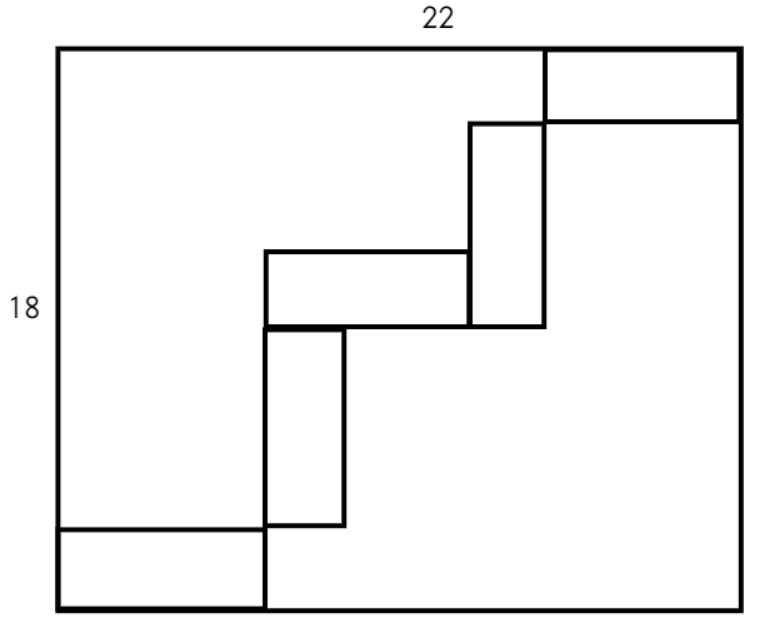
\includegraphics[scale=0.35]{nest7-112.png}}
\end{figure}\\
113. Для натуральных чисел $a,\ b,\ c$ верно равенство $a+\cfrac{1}{b+\cfrac{1}{c}}=\cfrac{35}{11}.$ Чему может быть равно $abc?$\\
114. Найдите все пары натуральных чисел, удовлетворяющих условию $(x-2y)(x-3)=6.$\\
115. Сколько среди чисел 30303032, 246801, 56781234, 67812345 точных квадратов?\\
116. Сумма квадратов цифр трёхзначного числа равна 101. Если из этого числа вычесть 198, то получится трёхзначное число, записанное теми же цифрами, но в обратном порядке. Каким было исходное число?\\
117. Найдите наименьшее натуральное число, большее 6, остатки от деления которого и на 7, и на 17 равны 6. Не забудьте обосновать свой ответ.\\
118. Найдите наименьшее натуральное число, большее 4, остатки от деления которого и на 5, и на 19 равны 4. Не забудьте обосновать свой ответ.\\
119. Вычислите: $\cfrac{1}{6}\cdot 7^{32}-(7+1)(7^2+1)(7^4+1)(7^8+1)(7^{16}+1)=?$\\
120. Вычислите: $\cfrac{1}{4}\cdot 5^{32}-(5+1)(5^2+1)(5^4+1)(5^8+1)(5^{16}+1)=?$\\
121. Известно, что для некоторого натурального $n$ дробь $\cfrac{n - 5}{2n - 1}$ --- целая. Чему она может быть
равна?\\
122. Известно, что для некоторого натурального $n$ дробь $\cfrac{n - 1}{2n - 5}$ --- целая. Чему она может быть
равна?\\
123. Имеется 12 сосисок длиной $X$ см каждая. Их требуется разделить между $X$ котятами, $X$ кошками и $X$ котами так, чтобы каждому котёнку достался кусок сосиски длиной 3 см, каждой кошке ---
кусок сосиски длиной 4 см, а каждому коту --- кусок сосиски длиной 5 см. Можно ли это сделать, если а) $X = 14;$ б) $X = 11?$\\
124. Имеется 10 сосисок длиной $X$ см каждая. Их требуется разделить между $X$ котятами, $X$ кошками и $X$ котами так, чтобы каждому котёнку достался кусок сосиски длиной 2 см, каждой кошке ---
кусок сосиски длиной 3 см, а каждому коту --- кусок сосиски длиной 5 см. Можно ли это сделать, если а) $X = 14;$ б) $X = 11?$

ewpage
